\section{General}
Predictive analytics (PA) is a broad field of applied mathematics. First, it includes all the statistical models and empirical methods that are used to create empirical predictions. Second, also predictive power, that is, methods for assessing the quality of predictions is a part of PA. \cite{Shmueli10} Another purpose of PA is to guide theory building, theory testing and relevance assessment. \cite{Dubin69}

One way to classify PA methods is to divide them into predictive models, descriptive models and decision models. Predictive models look for the most significant explanatory variables with which they are able to predict the dependent variables. Descriptive models, in turn, try to find as many relationships as possible, leading to segmented models that describe the world as it is. Decision models use optimization techniques to find the most optimal decision based on possible outcomes. \cite{Fico06}

Another way to classify PA methods is to distinguish between methods that predict the present and methods that shape the future. Predicting the present means applying patterns of current behavior with as much historic data as possible. These methods use classification, regression, clustering and all data mining techniques to predict similar occurrences in the future. Shaping the future has to do with generating new standards after the underlying assumptions have changed. While predicting the present can be thought as fitting a curve into the existing data, shaping the future creates a totally new curve with new assumptions and anticipated behaviors. \cite{Oracle10} In this thesis, all the used methods can be classified as predicting the present.

The methods of PA can also be divided into regression and machine learning  techniques. The simplest model is probably linear regression, which tries to find a linear model between a set of independent variables and a dependent variable by minimizing the squared error \cite{Montgomery12}. Time series models assume that the process we are investigating has some kind of internal structure with autocorrelation, trend or seasonal variation. This structure may be discovered with either time-domain or frequency-domain analysis. \cite{Hamilton94} The former is based on auto-correlation and cross-correlation analysis, while the latter is carried out with spectral or wavelet analysis, which I will talk about more in chapter 3.5.

Machine learning algorithms form a model, based on clustering or historic data, that is able to predict the class of the dependent value without necessarily knowing the exact mathematical structure behind it. As an example of clustering based methods, unsupervised Artificial Neural Networks (ANNs) are biology-inspired complex networks that evolve into a form that can classify new instances into a group with the most similar instances. \cite{Mitchell97} Models based on historic data are called supervised models and they can, for example, find a classifier function that separates the training data most effectively. I will talk more about classifiers in chapter 3.5 when I introduce Support Vector Machines.



\section{Combining CEP and PA}

The work of Fulop et al. \cite{Fulop12} lists several synergies and differences of CEP and PA which are briefly summarized in this section. 

Complex event processing (CEP) and Predictive Analytics (PA) are similar in the sense that they try to somehow make sense of large datasets, either in real-time or from historic data. The biggest differences between CEP and PA stem from the timing of the reasoning process. While CEP processes data real-time and detects the events only after they have occurred, PA, as the name suggests, tries to predict events by detecting the patterns that lead to them. 

\begin{figure}[here]
\centering
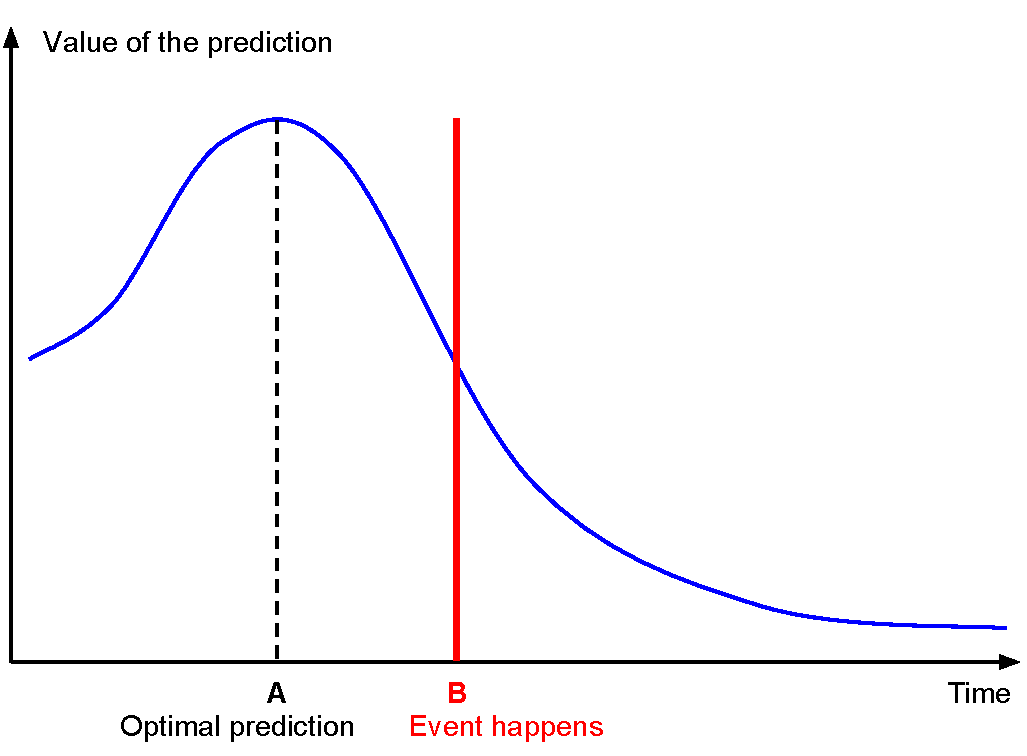
\includegraphics[scale=0.7]{images/prediction_value_v2.pdf}
\caption{Expected value of event detection as a function of time. An optimal prediction is made at the point A. The event happens at the point B, after which detecting the event is still valuable.}
\label{fig:prediction_value}
\end{figure}

The (expected) value of detecting an event depends directly on time, which is illustrated in Figure~\ref{fig:prediction_value}. Up to point A, value increases with increased accuracy. This is because long time predictions are not usually accurate. Nevertheless, since an early prediction is more useful than one that is made just a few seconds before, the value begins to fall rapidly. After the point B where the event actually happens, detecting an event is still useful and the value decreases slowly. The optimal prediction point A in Figure~\ref{fig:prediction_value} motivates this thesis' search for a predictive event processing model.

Another difference between CEP and PA is the need for building rules that detect patterns. CEP relies heavily on predefined rules that have to be implemented by a domain expert that knows the complex event in question. This can be considered a weak point of CEP. PA, in turn, aims at automating the rule creation. Of course, PA methods need to be implement, too, but that happens before the model is crafted into a certain scenario. The model should then adapt to different kinds of scenarios. In CEP a specialized model is required for each different scenario.

There are several requirements that should be taken into consideration when designing a predictive CEP system. First, CEP and PA components must be able to communicate with each other so that CEP receives Primary Complex Event (PCE) predictions from PA and PA receives predictors from CEP. Second, integrating the PA component should not affect the existing CEP part nor its maintainability in any way. \cite{Fulop12}

There are two ways to overcome these requirements. The first is to introduce predictive event processing agents (PEPAs) into the Event Processing Network (EPN). The second is to create a separate predictive event processing network (PEPN) that is somehow connected to the original EPN. Only the latter of these options satisfied the condition that the original EPN should not be affected in any way. The maintainability of EPN suffers greatly if PEPAs are mixed with original EPAs. \cite{Fulop12} The implementation chapter describes how this requirement is actually fulfilled. 


\section{Predicting with Time Series Classification}
Our task is to predict whether or not a certain event will happen in a defined time period in the future. Figure~\ref{fig:prediction_time_span} shows an outline of this process. Let's assume that the complex event we are trying to predict occurs between $t_{E,1}$ and $t_{E,2}$. Then, in order to gain advantage from predictive analytics, the prediction should happen before the warning time begins at $t_{P,2}$. We can define a prediction time period to be the interval from $t_{P,1}$ to $t_{P,2}$, which contains the event history available for making the prediction. Thus, we can assume that the prediction happens at $t_{P,2}$ and uses information from $t_{P,1}$ to $t_{P,2}$. In Chapter 4 I will discuss how to choose the interval lengths 

\begin{eqnarray}
\textbf{windowLength} &=& t_{P,2} - t_{P,1} \\
\textbf{waitingInterval} &=& t_{E,1} - t_{P,2} \\ 
\textbf{eventInterval} &=& t_{E,2} - t_{E,1} 
\end{eqnarray}

\begin{figure}[here]
\centering
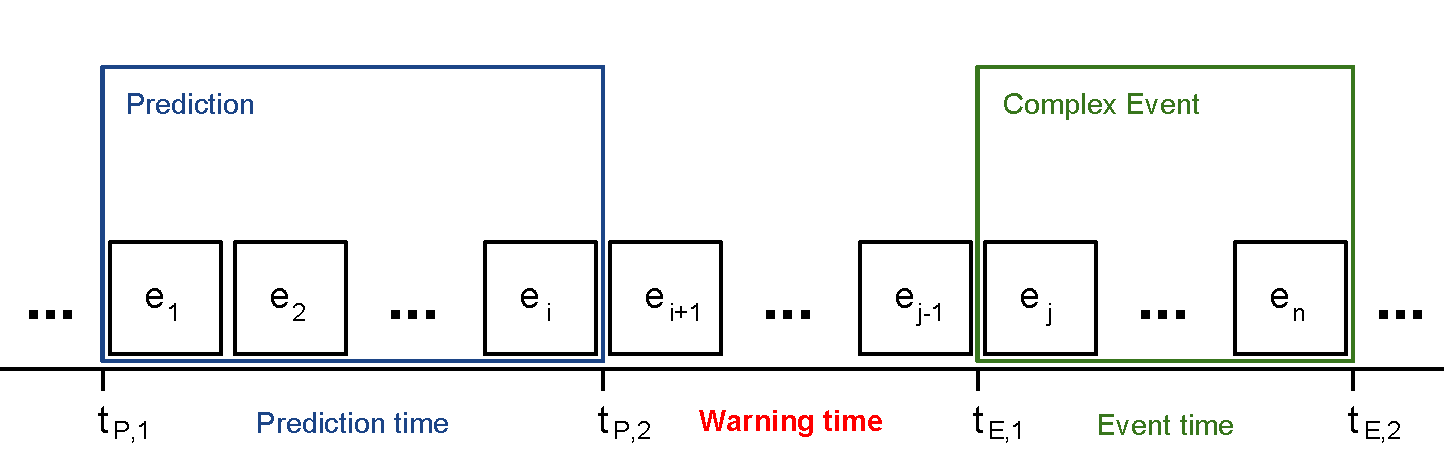
\includegraphics[scale=0.7]{images/prediction_time_span.pdf}
\caption{Timing of complex event prediction.}
\label{fig:prediction_time_span}
\end{figure}

The event history $h = \{e_1, ..., e_i\}$ in the prediction interval is a multivariate time series, that is, it contains a sequence of numerical vectors. \cite{Xing10} Each vector contains the measurement values from different sensor at a certain point in time. I will design the system so that the CEP engine receives every $\Delta t$ seconds a new event that contains the recent measurement values from all the available sensors. The choice of $\Delta t$ depends on the phenomenon investigated, an issue which I will talk about more in Chapter 4.

We can formulate the prediction process as a binary classification task that contains two classes:
\begin{enumerate}
\item{Histories that precede an event}
\item{Histories that do not precede an event}
\end{enumerate} 

We can denote theses classes by $w_1$ and $w_2$.
The task is to learn a classifier $C$, which maps a history $h$ into a class $w$: $C \ : \ h \rightarrow w, \ w \in C$, where 
\begin{eqnarray*}
C &=& \{w_1, w_2\} \label{eq:classification} \\
&=& \{\text{``Event is not going to happen''}, \text{``Event is going to happen''}\}
\end{eqnarray*}

Time series classification methods can be divided into different categories: distance based methods, feature based methods, model based methods and so on. Two of these, distance based and feature based methods are investigated and tested in this thesis. 

From distance based methods I present $L_p$ norms and Dynamic Time Warping (DTW) as distance measures in co-operation with k-Nearest Neighbor (kNN) and Learning Vector Quantization as classification methods. The empirical section of this thesis employs a model that uses DTW and kNN.

From feature based methods I present Fourier and Wavelet analyses for feature extraction and then Support Vector Machines (SVMs) for classifying the feature vectors.



\section{Distance Based Time Series Classification}
Distance based methods are probably the simplest way to classify time series. They rely on a measure function that relates the time series to a single numeric value which indicates the similarity between two different time series. Then, a classification method can be used to separate different classes of time series. \cite{Xing10}

In this chapter I first present $L_p$ norms and Dynamic Time Warping (DTW) as examples of measure functions. Then, k-nearest neighbors (kNN) and learning vector quantization (LVQ) algorithms are formulated for classifying the time series.



\subsection{$L_p$ norms}
One way to classify time series is to calculate a distance measure between a new time series and the existing labeled time series. Then, one can select the group with has the lowest distance with the time series being classified. The easiest approach is some $L_p$ norm which can be calculated for time series $\mathbf{x} = \{x_0, x_1, ..., x_{n-1}\}$ and $\mathbf{y} = \{y_0, y_1, ..., y_{n-1}\}$ with \cite{smith07}

\begin{equation}
D(\mathbf{x}, \mathbf{y}) = \left( \sum_{i=0}^{n-1} \left| x_i - y_i \right|^p \right)^{\frac{1}{p}}.
\end{equation}

Then, one can use various algorithms, such as nearest neighbor classifiers or decision trees, to classify the time series into different groups. Examples of $L_p$ norms are Manhattan norm ($p = 1$), Euclidean norm ($p = 2$) and maximum norm ($p \rightarrow \infty$). $L_p$ norms are very straightforward to calculate but requires normalization of the signals in order to handle similar signals with different amplitudes. \cite{MiningTimeSeriesData} 

\subsection{Dynamic Time Warping}
$L_p$ norms cannot group signals that are, for example, in different phases, no matter how similar they are. One way to overcome this problem is to use dynamic time warping (DTW) algorithm. It measures the similarity between two signals that may vary in time or speed by "warping" the axis of one time series so that the phases of the signals match. \cite{MiningTimeSeriesData} Let us denote a feature space, that is, available values for $x_i$ and $y_j$ by $\digamma$. A classical DTW algorithm begins by creating a matrix 

\begin{equation}
C(i, j) = c(x_i, y_j),
\end{equation}
where $c$ is a local distance measure: $c \ : \ \digamma \times \digamma \rightarrow \mathbb{R}$ that is the difference between the two variables. In other words, the two time series being compared are laid on the two axes of the matrix and the matrix contains the differences between the corresponding values in the time series.

Then, by using dynamic programming, a monotonically increasing minimal path from the bottom left corner of the matrix to the top right corner is searched. The algorithm begins by calculating the cumulative matrix \emph{D} beginning from the bottom left corner of the cost matrix \emph{C}. Then, the minimum path in the cumulative matrix defines the optimal alignment between \emph{x} and \emph{y}. \cite{Muller07} 

The difference between Euclidean distance and DTW distance is illustrated in Figure~\ref{fig:euclidean_vs_dtw}. While Euclidean distance always compares the two time series point by point, DTW distance warps the other time series so that the extrema of the two time series are matched. This gives a more comprehensive similarity measure for two time series.

\begin{figure}[here]
\centering
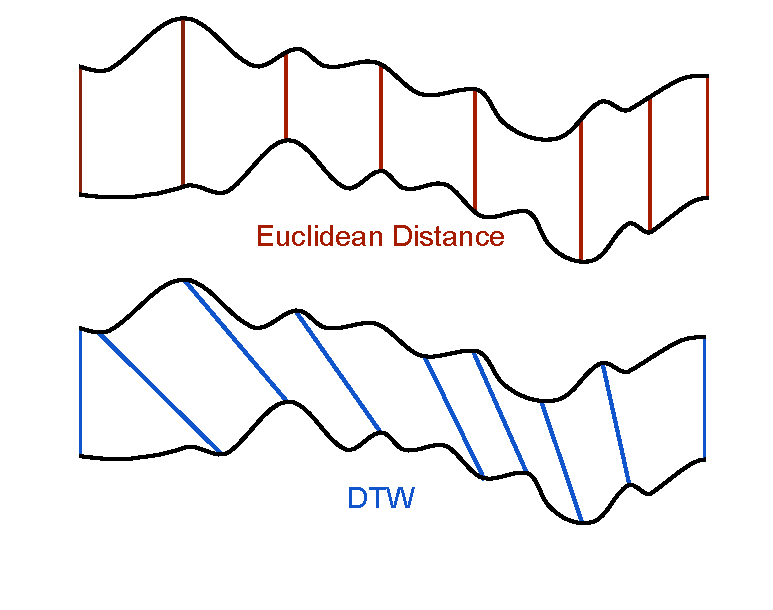
\includegraphics[scale=0.7]{images/euclidean_vs_dtw.pdf}
\caption{Difference between Euclidean Distance and Dynamic Time Warping.}
\label{fig:euclidean_vs_dtw}
\end{figure}



The vertical lines in the figure illustrate the points in the time series that are compared against each other. As can be seen, the algorithm matches the peaks and the valleys with one another. A pseudo code is presented in the following:


\begin{algorithm}[H]
	\KwData{Cost function $c$, Width $N$, Height $M$}
	\KwResult{Optimal Warping Path $p$}	
	Calculate cumulative cost matrix D starting from bottom left corner\;
	Set n = N and m = M\;
	\While{n > 0 and m > 0}{
		Move to neighbor with the smallest D(n, m)\; 
		Store movement to p\;
		Update n and m\;
	}
	reverse $p$\;
	return $p$;
\end{algorithm}


\subsection{k-Nearest Neighbor Algorithm}
Our classifying task consists of two classes as shown in Equation~\ref{eq:classification}. Once we have agreed on which distance measure we are using, we can use k-nearest neighbor (kNN) algorithm to classify new time-series instances. In the experimental chapter of this thesis I use Dynamic Time Warping (DTW) that was introduced in the previous section.

The kNN algorithm is a supervised learning algorithm, which means that we need a labeled teaching set to initialize the algorithm. \cite{PatternRecognition} The time-series in the teaching set have been labeled so that their label is either $w_1$ or $w_2$ depending on which class they belong to. 

Now for every new time-series instance we calculate the distance between the new instance and all the instances in the teaching set. Then, we select the $k$ instances with the least distances to our new instance. These $k$ instances vote for how the new instance is classified: the class with most instances is chosen. Clearly, the parameter $k$ should be odd so that we avoid draws between the two classes. \cite{Hastie08}


\subsection{Learning Vector Quantization}
Learning vector quantization (LVQ) is a supervised neural network that uses winner-take-all prototype-based learning. The LVQ algorithm, first developed by Teuvo Kohonen \cite{Kohonen90}, is similar to the kNN except for the application of moving prototype vectors. The M prototype vectors $\{z_1, ..., z_M\}$ are labeled vectors that represent the classes $C(z_m), m = 1, 2, ..., M$ and can be selected randomly from the set of available training vectors. Then, for each training vector $x_i, i = 1, ..., N$ the nearest prototype vector $z_m$ is updated with the following rule:
\begin{align}
z_m \leftarrow 
\begin{cases}
z_m + \alpha (x_i - z_m), & \text{if $z_m$ and $x_i$ belong to the same class} \\
z_m - \alpha (x_i - z_m), & \text{if $z_m$ and $x_i$ belong to different classes}
\end{cases},
\end{align} 

where $\alpha$ is the learning rate. In other words, the closest prototype vector is moved towards the instance if its from the same class as the prototype vector. In the opposite case, the prototype vector is moved away from the instance. When using the model with testing data, each new instance is classified with the same class as the closest prototype vector.

Usually, the training vectors are iterated through multiple times for a better convergence. On every iteration the value of $\alpha$ can be decreased so the algorithm first takes larger steps and then gradually moves to smaller steps. By doing this it first moves the prototype vectors to correct areas and then refines their positions. \cite{Li08}



\section{Feature Based Time Series Classification}
The aim of feature generation is to transform a sequence of time series data into a single vector that has as few dimensions as possible but still contains the relevant information about the time series for the classifying task. This process is a part of the preprocessing step of machine learning. We do this in order to reduce dimensionality, to increase learning accuracy and to improve result comprehensibility. \cite{Yu03}

There is a clear difference between feature selection and feature extraction. The former means choosing a subset from the available variables and using that as a feature vector, which is not an applicable method in the case of a time series as each variable in our multivariate time series is of a too high dimensionality by itself. The latter means mapping the available data into a lower dimensional space with some algorithm. \cite{Yu03} In sections 3.5.1 and 3.5.2 I present a technique for feature extraction by capturing a subset of the signal spectra with wavelet analysis.

Theoretically we could combine all the time series vectors from the prediction interval into one large feature vector that is then used as an input for the classifier $C$. However, as the prediction interval gets longer, we face the curse of dimensionality. The longer the feature vector is, the sparser the data becomes and the less statistically significant the classifying is. Also, the volume of the data increases rapidly and the processing becomes more and more demanding. \cite{Pascual07} For this reason, I describe a way to reduce the dimensionality of the feature vectors.

\subsection{Wavelet Analysis}
Wavelet analysis is a generalization of Fourier analysis which breaks the signal into series of sines and cosines. This transformation reveals the frequency space properties but loses all the temporal information. \cite{Fong04} A Fourier transform of a function $x(t)$ is 
\begin{equation}
F_{x}(t) = a_0 + \sum_{k=1}^{\infty} a_k cos(kt) + b_k sin(kt),
\end{equation}

where
\begin{align}
a_0 &= \frac{1}{2\pi} \int_{0}^{2\pi} x(t) dt \\
a_k &= \frac{1}{\pi} \int_{0}^{2\pi} x(t) cos(kt) dt \\
b_k &= \frac{1}{\pi} \int_{0}^{2\pi} x(t) sin(kt) dt.
\end{align}

This corresponds to a mapping into the frequency space that is formed by orthogonal basis functions, sine and cosine. By orthogonality we mean that for a set of signals $\psi_n(t)$, $-\infty < n < \infty$, we have
\begin{equation}
\left \langle \psi_n(t), \psi_m(t) \right \rangle = 0, \; m \ne n
\end{equation}

We can generalize the idea of Fourier transform into any orthogonal basis of signals $\psi_n(t)$. The analysis part calculates the coefficients of the original signal $x(t)$ in the new space:
\begin{equation}
c_n = \frac{\left \langle x(t), \psi_n(t) \right \rangle}{\left \langle \psi_n(t), \psi_n(t) \right \rangle}.
\end{equation}

Then, the original signal can be constructed from the coefficients by
\begin{equation}
x(t) = \sum_{n=-\infty}^{\infty} c_n \psi_n(t),
\end{equation}
which is called the synthesis process.

Fourier transform reveals the frequency band of the signal while losing all the temporal information about different frequencies. \cite{Fong04} Because of this Fourier transform is applicable only to stationary signals $f(t)$ whose variance does not vary with time. No information about the changes in variance are captured by Fourier transformation and hence the method becomes useless with non-stationary signals. Anomalies in time series data cause spectral variance and hence the signal is not stationary. \cite{Hautakangas11} 

We can define the short time Fourier transform (STFT) as
\begin{equation}
\operatorname{STFT}(f, s) = \int_{-\infty}^{\infty} x(t) g(t-s) e^{-j 2\pi ft} dt,
\end{equation}
where $f$ is frequency of $x(t)$ and $g(t)$ is a sliding window function, for example, a box function
\begin{equation}
\operatorname{box}(t) = 
\begin{cases}
1 & \text{for} \; |t| \le 1/2 \\
0 & \text{elsewhere}
\end{cases}.
\end{equation}

This restricts the Fourier transform into one window at the time and thus achieves time-localization which the ordinary Fourier transform lacks of. For computational purposes we must discretize this by denoting $f_n = n/T$ and $s_m = mT$. In this case our orthogonal basis functions are
\begin{equation}
v_{n,m} (t) = e^{j 2\pi nt / T} g(t - mT).
\end{equation}

Now the analysis part is
\begin{align}
c_{n,m} &= \frac{\left \langle x(t), v_{n,m}(t) \right \rangle}{\left \langle v_{n,m}(t), v_{n,m}(t) \right \rangle} \\
&= \frac{1}{T} \int_{mT}^{(m+1)T} x(t) e^{-j 2\pi nt / T} dt
\end{align}
and the synthesis is 
\begin{equation}
x(t) = \sum_{n=-\infty}^{\infty} \sum_{m=-\infty}^{\infty} c_{n,m} e^{j 2\pi nt / T} g(t - mT).
\end{equation}

Unlike Fourier transform, wavelet transformation gives the signal localization in both time and frequency spaces. It does this by using a concept called multi-resolution analysis (MRA) which means that different frequencies are analyzed with different resolutions. While Fourier transformation uses equally-sized windows for all frequencies, Wavelet transformation uses longer time windows for low frequencies and shorter time windows for high frequencies. This approach allows good localization of high frequency components while preserving information about low frequency contents of the signal. \cite{Fong04}

Continuous wavelet transform (CWT) for signal $x(t)$ is defined as
\begin{equation}
C_{x}(a,b) = \frac{1}{\sqrt{|a|}} \int_{-\infty}^{\infty} x(t) w \left ( \frac{t - b}{a} \right ) dt,
\end{equation}
where $a$ and $b$ are scaling and positioning parameters and $w(t)$ is a so-called mother wavelet function. \cite{Fong04} 

For computational purposes we must find a discrete wavelet transform (DWT). By choosing the scales to be powers of 2 and the positions to be multiples of the scales, we get an orthogonal basis of functions for CWT:
\begin{equation}
w_{j,k}(t) = 2^{j/2} w(2^j t - k).
\end{equation}

These $w_{j,k}(t)$ are called the baby wavelets. \cite{Phillips03} As can be easily seen, baby wavelets become narrower and higher as the $j$ increases. The reverse is also true, baby wavelets become wider and flatter as the $j$ decreases. We can now define space $W_j$ to contain all the signals $x_j(t)$ that can be synthesized from baby wavelets $w_{j,k}(t)$ with the $j$ fixed:
\begin{equation}
x_j(t) = \sum_{k=-\infty}^{\infty} c_{j,k} w_{j,k}(t).
\end{equation}

Similarly, let $V_j$ to be the space of signals $x(t)$ that can be synthesized from baby wavelets $w_{i,k}(t)$ where $i < j$ and $-\infty < k < \infty$. Then, from the definition of $W_j$ and $V_j$ we have $V_{j+1} = W_j + V_j$. This is illustrated in figure~\ref{fig:wavelet_spaces}.


\begin{figure}[here]
\centering
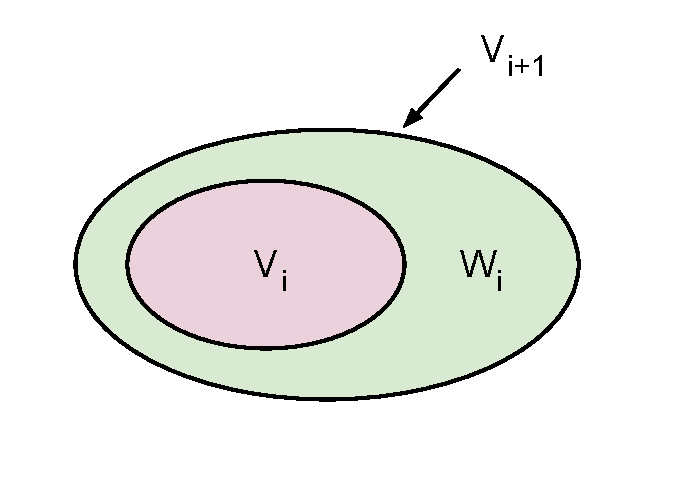
\includegraphics[scale=0.7]{images/wavelet_spaces.pdf}
\caption{Wavelet subspaces.}
\label{fig:wavelet_spaces}
\end{figure}

Thus, the spaces $V_j$ are nested inside each other, that is $\{0\} \subset \ldots \subset V_{-1} \subset V_{0} \subset V_{1} \subset \ldots L^2$, where $L^2$ contains all possible signals. The spaces $W_j$ are the differences between adjacent spaces $V_j$ and $V_{j+1}$. Now we can divide the space $V_0$ as
\begin{align*}
V_0 &= V_{-1} + W_{-1} \\
&= V_{-2} + W_{-2} + W_{-1} \\
&= V_{-3} + W_{-3} + W_{-2} + W_{-1} \\
&= \cdots
\end{align*}
and the signal as
\begin{align}
x(t) &= A_1(t) + D_1(t) \label{eq:decomposition} \\
&= A_2(t) + D_2(t) + D_1(t) \\
&= A_3(t) + D_3(t) + D_2(t) + D_1(t) \\
&= \cdots,
\end{align}
where $D_i(t) \in W_{-i}$ is the detail at level $i$ and $A_i(t) \in V_{-i}$ is the approximation at level $i$. This approach is called multi-resolution analysis (MRA) because on each step we divide the frequency band into two pieces and then continue the process on the lower half. At each stage the $A_i(t)$ corresponds to low-pass filtered signal and the $D_i(t)$ to high-pass filtered signal. This way we get more detailed information about the high frequencies. \cite{Phillips03} 

To facilitate the computations we can define a scaling function $\phi(t)$ (sometimes called the father wavelet) which produces the subspaces $V_j$:
\begin{equation}
\phi_{j,k}(t) = \sqrt{2^j} \phi(2^j t - k).
\end{equation}

Because $V_0 \subset V_1$ and $W_0 \subset V_1$, it is possible to construct the mother wavelet and the scaling function in $V_1$ from the scaling function in $V_0$ as follows
\begin{align}
\phi(t) &= \sum_n h_0(n) \sqrt{2} \phi(2t - n) \\
w(t) &= \sum_n h_1(n) \sqrt{2} \phi(2t - n),
\end{align}
where $h_0(n)$ and $h_1(n)$ are discrete time filter coefficients. These depend on the choice of wavelet type and they will be defined later. Now we are able to define the signal $x(t) \in V_j$ using the mother wavelet and the scaling function in spaces $V_{j-1}$ and $W_{j-1}$
\begin{align}
x(t) &= \sum_k cA_0(k) \phi_{j,k}(t) \\
&= \sum_k cA_1(k) \phi_{j-1,k}(t) + \sum_k cD_1(k) w_{j-1,k}(t) \\
&= A_1(t) + D_1(t),
\end{align}
where $cA_0(k)$, $cA_1(k)$ and $cD_1(k)$ are the approximate and detail coefficients respectively. Then, $\phi_{j-1,k}$ can be further filtered to get the next level signals as shown in equation~\ref{eq:decomposition}. The coefficient values can be derived as follows
\begin{align}
cA_1(k) &= \left \langle x(t), \phi_{j-1,k}(t) \right \rangle \\
		&= \left \langle \sum_n cA_0(n) \phi_{j,n}(t), \phi_{j-1,k}(t) \right \rangle \\
		&= \sum_n cA_0(n) \left \langle \phi_{j,n}(t), \phi_{j-1,k}(t) \right \rangle,
\end{align}
which, by calculating the inner product simplifies to
\begin{align}
cA_1(k) = \sum_n h_0(n-2k) cA_0(n)
\end{align}

Similarly, for $cD_1(k)$ we get
\begin{align}
cD_1(k) = \sum_n h_1(n-2k) cA_0(n)
\end{align}

These two operations correspond to filters
\begin{align}
&cA_0(n) \longrightarrow \boxed{h_0(-n)} \longrightarrow \boxed{\downarrow 2} \longrightarrow cA_1(k) \label{eq:downsampling1} \\
&cA_0(n) \longrightarrow \boxed{h_1(-n)} \longrightarrow \boxed{\downarrow 2} \longrightarrow cD_1(k), \label{eq:downsampling2}
\end{align}
where the downsampling filter, $\boxed{\downarrow 2}$, means omitting every other value from the signal. As shown in equation~\ref{eq:decomposition}, we can further use the downsampling filters to decompose the signal into more detail. This process is shown in Figure~\ref{fig:wavelet_filters}.

\begin{figure}[here]
\centering
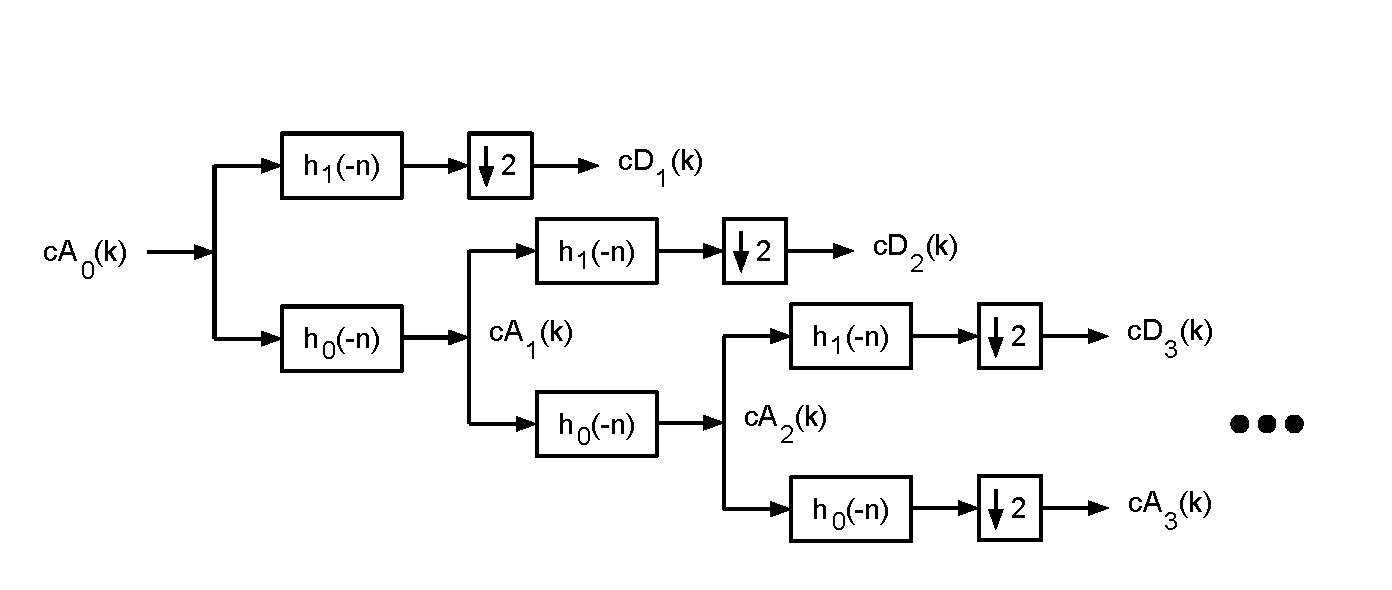
\includegraphics[scale=0.7]{images/wavelet_filters.pdf}
\caption{Wavelet coefficient decomposition using filters.}
\label{fig:wavelet_filters}
\end{figure}

Now on level $N$ our coefficients are
\begin{align}
C = [cA_N, cD_N, cD_{N-1}, ..., cD_2, cD_1]
\end{align}

The signal is now compressed by setting some of the detail coefficients to zero. Of course, the energy of the signal is not completely preserved and the number of zero coefficients depends on the application.

Next, we need to perform the synthesis part by opposite, upsampling filters. This process is shown in Figure~\ref{fig:wavelet_filters2}.

\begin{figure}[here]
\centering
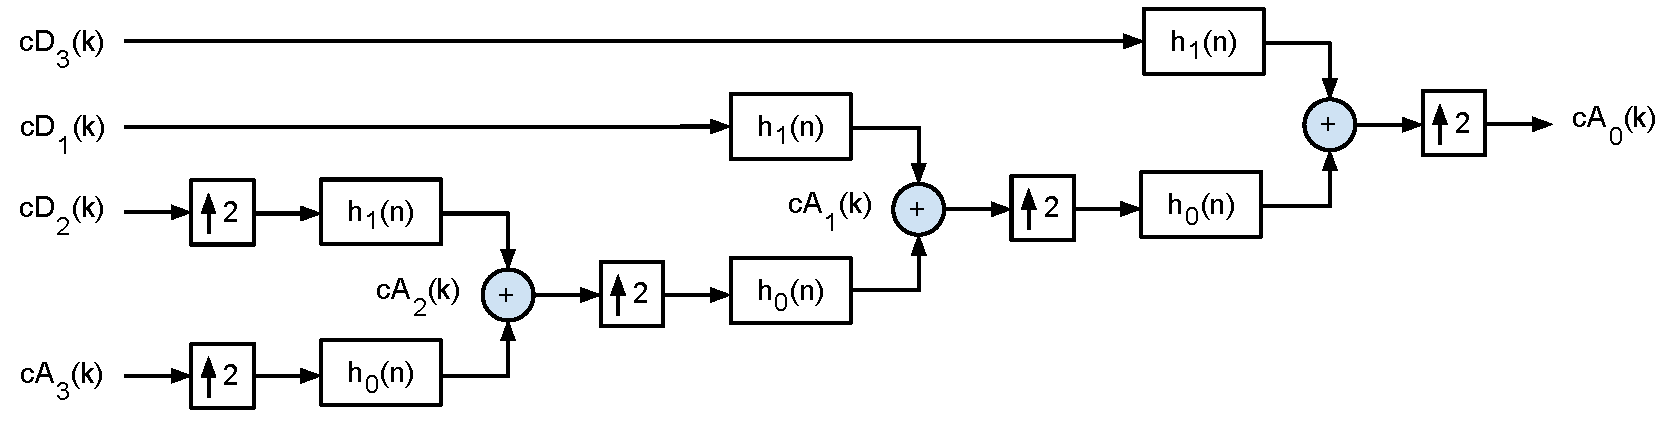
\includegraphics[scale=0.55]{images/wavelet_filters2.pdf}
\caption{Wavelet coefficient decomposition using filters.}
\label{fig:wavelet_filters2}
\end{figure}

If no coefficients are set to zero in the analysis phase, the signal that is constructed in the synthesis phase is exactly the same as the original signal. By setting some of the detail coefficients to zero before the synthesis, some energy of the signal is lost but at the same time the signal is compressed to a smaller size.


\subsection{Haar Wavelet Decomposition for Time Series}
Haar wavelet \cite{struzik99} is the simplest possible wavelet and it has the following mother wavelet 
\begin{align}
\psi(t) = 
\begin{cases}
1, & 0 \le t < 1/2 \\
-1, & 1/2 \le t < 1 \\
0, & otherwise
\end{cases}.
\end{align}

and the following scaling function
\begin{align}
\phi(t) = 
\begin{cases}
1, & 0 \le t < 1 \\
0, & otherwise
\end{cases}.
\end{align}

For Haar wavelets the discrete time filter coefficients $h_0(n)$ and $h_1(n)$ are defined as
\begin{align}
h_0 &= \left [ \frac{1}{\sqrt{2}}, \frac{1}{\sqrt{2}} \right ] \\
h_1 &= \left [ \frac{1}{\sqrt{2}}, -\frac{1}{\sqrt{2}} \right ].
\end{align}

Now let's assume we have a time-series $\mathbf{x} = (x_1, x_2, ..., x_N)$ of length $N = 2^n$. The 1-level Haar-Transform is
\begin{align}
\mathbf{x} \longleftrightarrow (A_1 | D_1),
\end{align}
where 
\begin{align}
A_1 &= \left ( \frac{x_1 + x_2}{\sqrt{2}}, \frac{x_3 + x_4}{\sqrt{2}}, ..., \frac{x_{N-1} + x_N}{\sqrt{2}} \right ) \\
D_1 &= \left ( \frac{x_1 - x_2}{\sqrt{2}}, \frac{x_3 - x_4}{\sqrt{2}}, ..., \frac{x_{N-1} - x_N}{\sqrt{2}} \right ).
\end{align}

The former operation corresponds to a running average (trend) and the latter to a running difference (fluctuation). Then, $A_1$ can be further decomposed into $A_2$ and $D_2$ by performing the same operation again:
\begin{align}
\mathbf{x} \longleftrightarrow (A_2 | D_2 | D_1).
\end{align}

This process is then repeated until a desired level is reached. The Wavelet can be compressed by setting some of the detail coefficients to zero. The resulting vector can now be used as a feature. In the next chapters I describe how these features can be classified with first linear classifiers and then with support vector machines (SVMs) that generalize into nonlinear cases.




\subsection{Linear Classifiers}
In this section I discuss the special case of linearly separable classes. If the input space is linearly separable, we can use a linear hyperplane to separate the two classes. \cite{tappen10} As explained in Chapter 3.3, we have two classes, $w_1$ and $w_2$, for which the $l$-dimensional hyperplane is

\begin{equation}
g(\mathbf{x}) = \mathbf{w}^T \mathbf{x} + w_0 = 0,
\end{equation}
where $\mathbf{x}$ is a feature vector, $\mathbf{w}$ is the weight vector, and $w_0$ is the threshold. The threshold value is needed to cover the case of the hyperplane not crossing the origin. We can extend the vectors into $(l+1)$-dimensional space by defining
\begin{eqnarray}
\mathbf{x'} = \left [ \mathbf{x}^T, 1 \right ]^T \\
\mathbf{w'} = \left [ \mathbf{w}^T, w_0 \right ]^T.
\end{eqnarray}

From now on the variables $\mathbf{x}$ and $\mathbf{w}$ refer to $\mathbf{x'}$ and $\mathbf{w'}$. Now the feature vectors $x$ have the properties
\begin{eqnarray}
\mathbf{w}^T \mathbf{x} > 0 &\;\;& \forall \mathbf{x} \in w_1 \\
\mathbf{w}^T \mathbf{x} < 0 &\;\;& \forall \mathbf{x} \in w_2.
\end{eqnarray}

The problem is now the choice of the weight vector $w$. One way to tackle the problem is the perception algorithm which defines a perception cost as
\begin{equation}
J(\mathbf{w}) = \sum_{\mathbf{x} \in Y} (\delta_x \mathbf{w}^T \mathbf{x}),
\end{equation}
where $Y$ is the set of training vectors that are misclassified with the weigh vector $w$ and $\delta_x = -1$ if $\mathbf{x} \in w_1$ and $\delta_x = +1$ if $\mathbf{x} \in w_2$. Since the cost $J(\mathbf{w})$ is always positive, continuous and piecewise linear, it can be minimized with a gradient descent method \cite{tappen10}:
\begin{eqnarray}
\mathbf{w(t+1)} &=& \mathbf{w(t)} - \rho_t \frac{\partial J(\mathbf{w})}{\partial \mathbf{w}} \\
&=& \mathbf{w(t)} - \rho_t \sum_{\mathbf{x} \in Y} \delta_x \mathbf{x}.
\end{eqnarray}

The iteration is performed until all the training instances have been classified correctly. A variation of perception algorithm loops through the training instances one by one and updates the weight vector on each instance.

Even though the classes are not linearly separable, we can find an optimal linear classifier that minimizes the classification error in some sense. One way to find the optimal $w$ is to use mean square error estimation which tries to minimize the cost function
\begin{equation}
J(\mathbf{w}) = E[|y - \mathbf{x}^T \mathbf{w}|^2],
\end{equation}  

where $y$ is the desired output; in this case $y = 1$ for $w_1$ and $y = -1$ for $w_2$. \cite{gutierrez11} A required condition for the minimum is
\begin{equation}
\frac{\partial J(\mathbf{w}}{\partial \mathbf{w}} = 2 E[\mathbf{x}(y - \mathbf{x}^T \mathbf{w})] = 0.
\end{equation}

The optimal weigh vector is then
\begin{equation}
\mathbf{w} = R_x^{-1} E[\mathbf{x}y],
\end{equation}
where $R_x$ is the correlation matrix of $\mathbf{x}$ and $E[\mathbf{x}y]$ is the cross-correlation vector that have to be estimated from the learning set.

Another way is to use least squares methods that use the cost function
\begin{equation}
J(\mathbf{w}) = \sum_{i=1}^N (y_i - \mathbf{x}_i^T \mathbf{w})^2 = \sum_{i=1}^N e_i^2
\end{equation} 

Then, by differentiating with respect to $\mathbf{w}$ we get
\begin{eqnarray}
&& \sum_{i=1}^N \mathbf{x}_i (y_i - \mathbf{x}_i^T \mathbf{w}) = 0 \\
&\Leftrightarrow& (\sum_{i=1}^N \mathbf{x}_i \mathbf{x}_i^T) \mathbf{w} = \sum_{i=1}^N (\mathbf{x}_i y_i) \\
&\Leftrightarrow& (\mathbf{X}^T \mathbf{X}) \mathbf{w} = \mathbf{X}^T \mathbf{y} \\
&\Leftrightarrow& \mathbf{w} = (\mathbf{X}^T \mathbf{X})^{-1} \mathbf{X}^T \mathbf{y},
\end{eqnarray}
where $\mathbf{X} = [\mathbf{x}_1, ..., \mathbf{x}_N]^T$, $\mathbf{y} = [y_1, ..., y_N]^T$, and $\mathbf{X}^T \mathbf{X}$ is sample correlation matrix which can be estimated from the available data. \cite{gutierrez11}




\subsection{Support Vector Machines for Linearly Separable Classes}
The following three chapters follow the support vector machine chapters 3.7 and 4.18 discussed in the book \emph{Pattern recognition} by Theodoridis and Koutroumbas \cite{PatternRecognition}.

I first discuss the Support Vector Machines in case of two linearly separable classes. Similarly to the previous section with linear classifiers, we design a hyperplane
\begin{equation}
g(\mathbf{x}) = \mathbf{w}^T \mathbf{x} + w_0 = 0
\end{equation}

\begin{figure}[here]
\centering
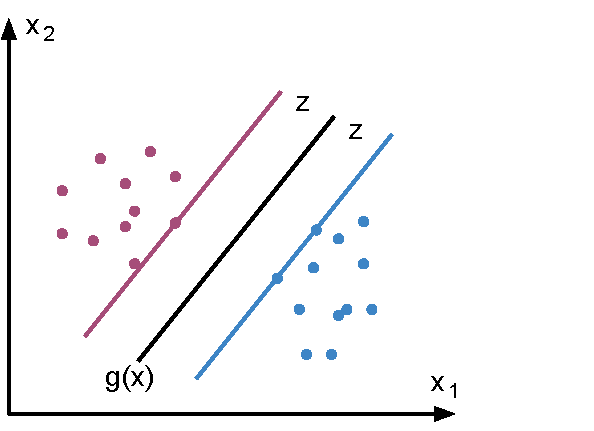
\includegraphics[scale=0.7]{images/svm_linear.pdf}
\caption{Maximum separating hyperplane between two linearly separable classes.}
\label{fig:svm_linear}
\end{figure}

When the hyperplane leaves maximal margins between the class instances and itself, the performance of classifier is optimal. This situation is depicted in Figure~\ref{fig:svm_linear}. Thus, we should maximize the margin $z$ which can be represented as $z = |g(\mathbf{x})| / ||\mathbf{w}||$. If we scale $\mathbf{w}$ and $w_0$ so that $g(\mathbf{x}) = 1$ for the class $w_1$ and $g(\mathbf{x}) = -1$ for the class $w_2$ on the points that are closest to the hyperplane, we have a margin of $2 / ||\mathbf{w}||$ and requirements
\begin{align}
\mathbf{w}^T \mathbf{x} + w_0 \ge 1, &\; \forall \mathbf{x} \in w_1 \\
\mathbf{w}^T \mathbf{x} + w_0 \le -1, &\; \forall \mathbf{x} \in w_2
\end{align}

We can form the problem as the following optimization problem
\begin{align}
\text{minimize} &\; J(\mathbf{w}, w_0) = \frac{1}{2} ||\mathbf{w}||^2 \\
\text{subject to} &\; y_i (\mathbf{w}^T \mathbf{x}_i + w_0) \ge 1, \; i = 1,2,...,N \label{eq:svm_linear_variables} 
\end{align}
where $y_1 = 1$ and $y_2 = -1$. The Karush-Kuhn-Tucker (KKT) conditions for this nonlinear quadratic optimization problem are
\begin{eqnarray} 
L_{\mathbf{w}}(\mathbf{w}, w_0, \mathbf{\lambda}) &=& \mathbf{0} \label{eq:KKT} \\
L_{w_0}(\mathbf{w}, w_0, \mathbf{\lambda}) &=& 0 \\
\lambda_i &\ge& 0, \; i = 1, 2, ..., N \\
\lambda_i [y_i (\mathbf{w}^T \mathbf{x}_i + w_0) - 1] &=& 0,
i = 1, 2, ..., N,
\end{eqnarray}
where $L(\mathbf{w}, w_0, \mathbf{\lambda})$ is the Lagrangian function
\begin{equation}
L(\mathbf{w}, w_0, \mathbf{\lambda}) = \frac{1}{2} \mathbf{w}^T \mathbf{w} - \sum_{i=1}^N \lambda_i [y_i (\mathbf{w}^T \mathbf{x}_i + w_0) - 1]
\end{equation}

Solving the first order differential equations in the KKT conditions yields a dual problem
\begin{eqnarray}
\text{maximize} &\;& L(\mathbf{w}, w_0, \lambda) \\
\text{subject to} &\;& \mathbf{w} = \sum_{i=1}^N \lambda_i y_i \mathbf{x}_i \\
&& \sum_{i=1}^N \lambda_i y_i = 0 \\
&& \mathbf{\lambda} \ge \mathbf{0}
\end{eqnarray}

By substituting the first two conditions into the Lagrangian $L$ we further get
\begin{eqnarray}
&\underset{\mathbf{\lambda}}{\operatorname{max}}& \left ( \sum_{i=1}^N \lambda_i - \frac{1}{2} \sum_{i, j} \lambda_i \lambda_j y_i y_j \mathbf{x}_i^T \mathbf{x}_j \right ) \label{eq:SVM_KKT_1} \\ 
&\text{subject to}& \sum_{i=1}^N \lambda_i y_i = 0 \label{eq:SVM_KKT_2} \\ 
&&\mathbf{\lambda} \ge 0 \label{eq:SVM_KKT_3}
\end{eqnarray}

As we can easily see, the function to be maximized does not depend on the dimensionality of the input space because it contains the input vectors in the form of a inner product. This allows us to easily generalize the method into non-separable classes by mapping them into a higher-dimensional space in the next sections.

The Support Vectors are the points $\mathbf{x}_i$ for which the Lagrangian multiplier $\lambda_i$ is not zero and which lie on one of the hyperplanes $\mathbf{w}^T \mathbf{x} + w_0 = \pm 1$. The optimal hyperplane of SVM is unique because the cost function in equation~\ref{eq:KKT} is strictly convex.


\subsection{Support Vector Machines for Linearly Non-separable Classes}
Now we turn to the case of classes that cannot be separated with a linear hyperplane. In this case we introduce slack variables $\xi_i \ge 0$ that allow some points to fall on the wrong side of the hyperplane. Now the equation~\ref{eq:svm_linear_variables} is replaced with
\begin{equation}
y_i [\mathbf{w}^T \mathbf{x} + w_0] \ge 1 - \xi_i,
\end{equation}  
where the value of $\xi_i$ defines the type of the point as follows:
\begin{enumerate}
\item $\xi_i = 0$ $\Rightarrow$ Point is classified correctly.
\item $0 < \xi_i \le 1$ $\Rightarrow$ Point is classified correctly but it is on the wrong side of the margin.
\item $\xi_i > 1$ $\Rightarrow$ Point is misclassified.
\end{enumerate}

These three types are illustrated in figure~\ref{fig:svm_non_separable}. An yellow ring marks a point that is classified correctly but that is on the wrong side of the margin (type 2). A red square marks a point that is misclassified (type 3).  

\begin{figure}[here]
\centering
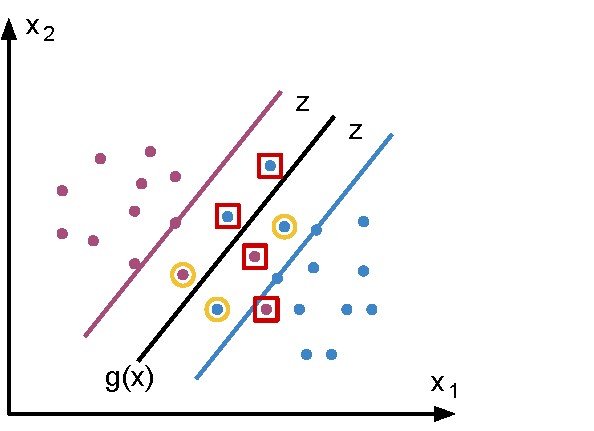
\includegraphics[scale=0.7]{images/svm_non_separable.pdf}
\caption{A separating hyperplane between two classes that are non-separable. A yellow ring marks a point that is classified correctly but that is on the wrong side of the margin. A red square marks a point that is misclassified.}
\label{fig:svm_non_separable}
\end{figure}

In this case our optimization problem can be stated as
\begin{align}
\text{minimize} &\; J(\mathbf{w}, w_0, \mathbf{\xi}) = \frac{1}{2} ||\mathbf{w}||^2 + C \sum_{i=1}^N I(\xi_i) \label{eq:SVM_C_parameter} \\
\text{subject to} &\; y_i [\mathbf{w}^T \mathbf{x}_i + w_0] \ge 1 - \xi_i, i = 1, 2, ..., N \\
& \xi_i \ge 0, i = 1, 2, ..., N,
\end{align}
where $I(\xi_i) = 1$ if $\xi_i > 0$ and $I(\xi_i) = 0$ if $\xi_i = 0$ and the parameter $C$ defines a trade-off between maximizing the margin and minimizing the number of misclassified points. Similarly to the previous section, we can build a dual problem that leads to the problem
\begin{align}
\underset{\mathbf{\lambda}}{\operatorname{max}} &\; \left ( \sum_{i=1}^N \lambda_i - \frac{1}{2} \sum_{i,j} \lambda_i \lambda_j y_i y_j \mathbf{x}_i^T \mathbf{x}_j \right ) \\
\text{subject to} &\; 0 \le \lambda_i \le C, i = 1, 2, ..., N \\
&\; \sum_{i=1}^N \lambda_i y_i = 0.
\end{align}

Again, the dimensionality of the input space disappears from the problem and the input vectors appear only as inner products. There is a shortcut for calculating these inner products with a kernel trick \cite{Jordan04}, which is described in the next section.

\subsection{Generalization of SVMs into Nonlinear Cases}
\begin{figure}[here]
\centering
\includegraphics[scale=0.7]{images/svm_mapping.pdf}
\caption{The main idea of Support Vector Machines. Classes are not linearly separable in the input space. They are mapped into a higher-dimensional space where a linear classifier can be formed. This classifier corresponds to a non-linear classifier in the original input space.}
\label{fig:svm_mapping}
\end{figure}


If the classes are not separable in the $l$-dimensional input space, we can find a mapping $\mathbf{x} \in \mathbb{R}^l \; \rightarrow \; \mathbf{y} \in \mathbb{R}^k$, where $k > l$. The choice of $k$ is done so that the original classes are linearly separable in the new, higher-dimensional space. This situation is depicted in Figure~\ref{fig:svm_mapping}. As mentioned in the previous chapters, our optimization problems contain input vector $x$ only as an inner product that is not altered by the mapping.

In order to present the Mercer's Theorem \cite{Jordan04} that relates the inner product to a kernel function, we need to explain some space related concepts. A Cauchy sequence is defined as a sequence $a_1, a_2, ...$ for which
\begin{equation}
\forall \epsilon \in \mathbb{R} \; \exists \; N > 0  \; s.t.  \; |a_m - a_n| < \epsilon, \; m, n > N
\end{equation}
In other words, the elements of the sequence become arbitrarily close as the sequence progresses. A complete space is a space where every Cauchy sequence converges to a point that is also contained within the space. A Hilbert space, in turn, is a generalization of Euclidean space into any finite or infinite number of dimensions. It is a complete vector space that has inner product defined for measuring lengths and angles. \cite{duchateau02}

Mercer's Theorem states that for each mapping $\mathbf{x} \rightarrow \mathbf{\phi}(\mathbf{x}) \in H$, where $H$ is a Hilbert Space, we have a kernel function $K(\mathbf{x}, \mathbf{y})$ that is equivalent for the inner product:
\begin{equation}
\left \langle \mathbf{\phi}(\mathbf{x}), \mathbf{\phi}(\mathbf{y}) \right \rangle = K(\mathbf{x}, \mathbf{y}).
\end{equation}

The kernel function must have the following properties
\begin{align}
\int_S \int_S K(\mathbf{x}, \mathbf{y})g(\mathbf{x})g(\mathbf{y})d\mathbf{x}d\mathbf{y} &\ge 0 \\ 
\int_S g(\mathbf{x})^2 d\mathbf{x} &< +\infty, \; \forall g(\mathbf{x}), \mathbf{x} \in S, 
\end{align}
where $S \subset \mathbb{R}^l$. The opposite is also true: for any Kernel function satisfying the conditions above there is a Hilbert space where the Kernel function is equivalent for the inner product. The problem is now how to find the mapping $\phi$ when we have selected the Kernel function.

Now we can replace the inner product in Equation~\ref{eq:SVM_KKT_1} with the Kernel function to get the optimization problem
\begin{align}
\underset{\mathbf{\lambda}}{\operatorname{max}} &\left ( \sum_i \lambda_i - \frac{1}{2} \sum_{i,j} \lambda_i \lambda_j y_i y_j K(\mathbf{x}_i, \mathbf{x}_j) \right ) \label{eq:SVM_final_problem} \\
\text{subject to} &\; 0 \le \lambda_i \le C, \; i = 1, 2, ..., N \\
&\; \sum_i \lambda_i y_i = 0.
\end{align}

The resulting non-linear classifier is then
\begin{equation}
g(\mathbf{x}) = \sum_{i=1}^{N_s} \lambda_i y_i K(\mathbf{x}_i, \mathbf{x}) + w_0 \begin{cases}
> 0, \; \Rightarrow \mathbf{x} \in w_1 \\
< 0, \; \Rightarrow \mathbf{x} \in w_2,
\end{cases} \label{eq:SVM_classifier}, 
\end{equation}
which is shown in Figure~\ref{fig:svm_network}. Input vectors enter the network from the left. Then, inner products are calculated in middle nodes, the number of which is N, the number of support vectors. An output node sums the components up and outputs a single real number that determines the result of the classification according to equation~\ref{eq:SVM_classifier}.


\begin{figure}[here]
\centering
\includegraphics[scale=0.7]{images/svm_network.pdf}
\caption{SVM classifier as a network. Input vectors enter the network from the left. Kernel functions calculate inner products in the middle nodes. Output node combines sums the components up and outputs a single real number.}
\label{fig:svm_network}
\end{figure}



\subsection{Using SVM for Time Series Analysis}
Before we can use our SVM classifier, we have to choose an appropriate kernel function $K(\mathbf{x}, \mathbf{y})$ for classifying wavelet based feature vectors. In literature one of the most used kernels is the Gaussian kernel \cite{Zhang04}, which is of the form
\begin{equation}
K(\mathbf{x}, \mathbf{y}) = \exp{\frac{||\mathbf{x} - \mathbf{y}||^2}{2\gamma^2}}, \label{eq:RBF_kernel},
\end{equation}
where $\beta > 0$ is a parameter chosen by the user. Gaussian kernel belongs to a family of functions called radial basis functions (RBF) whose value depends only on the distance between two points \cite{Scholkopf97}
\begin{equation}
f(\mathbf{x}, \mathbf{y}) = f(||\mathbf{x} - \mathbf{y}||)
\end{equation}

If we assume that the time series is generated by an AR(1)-process 
\begin{align}
x_T = g(x_{T-1}, ..., x_{T-k}) + \mu,
\end{align}
it can be shown that an ellipsoid with mean equal to the mean of the time series and variance equal to $\mu$ contains most of the data. The variable $\mu$ is a Gaussian noise component. Consequently, similar time windows are close to each other in the sense of Euclidean Distance. This makes RBF Kernels promising for time series analysis. \cite{Ruping01}

Another possibility is Polynomial Kernel that is of the form
\begin{equation}
K(\mathbf{x}, \mathbf{y}) = (\mathbf{x}^T \mathbf{y} + c)^d,
\end{equation}
which gives the Linear Kernel as a special case when $d = 1$. \cite{Scholkopf97}

Subsequence Kernels look for informative subsequences that are similar in dependent time windows. In this case the Kernel function becomes
\begin{equation}
K(\mathbf{x}, \mathbf{y}) = \sum_{s_x, s_y} K (s_x, s_y),
\end{equation}
where $s_x$ and $s_y$ are subsequences of x and y. There are $\binom{n}{k}^2$ possible combinations for time series of length $n$ and subsequence of length $k$, so one must use another algorithm for selecting the optimal subsequences. \cite{Ruping01}

In thesis I use Gaussian RBF Kernels because of their widespread use and good applicability to time series analysis. Ruping \cite{Ruping01} compared Linear, RBF, Fourier, Subsequence and Hidden Markov Model Kernels and came into conclusion that RBF Kernels perform very well on time series learning tasks. However, he recommends to investigate other possibilities in very specialized applications.

A well defined kernel function increases the performance of the SVM greatly and thus Kernel selection is an important part of SVM development \cite{Fong04}. In the case of RBF Kernels we must choose the value of $\gamma$ in \ref{eq:RBF_kernel}. From now on I try to find an optimal value for $\sigma$, which then defines the $\gamma$ from $\gamma = 1 / 2\sigma^2$. The value of $\sigma$ should be chosen so that it minimizes the error
\begin{equation}
E(\sigma) = \sum_{i=1}^N \left | g(\mathbf{x}_i, \sigma) - y_i \right |^2 \label{eq:SVM_error}
\end{equation}

A related theorem states that for a Support Vector Classifier (SVC) there exists a range $[\sigma_A, \sigma_B]$ for which
\begin{align}
&\forall \; \epsilon > 0 \;\; \text{and} \;\; \forall \; \sigma_1, \sigma_2 \in [\sigma_A, \sigma_B] \\
& \left | \sum_{i=1}^N \left | g(\mathbf{x}_i, \sigma_1) - y_i \right | - \sum_{i=1}^N \left | g(\mathbf{x}_i, \sigma_2) - y_i \right | \right | < \epsilon,
\end{align}
where $g(\mathbf{x}_i, \sigma_i)$ is the discriminant function from Equation~\ref{eq:SVM_classifier} and $y_i$ is the desired output ($\pm 1$) \cite{Wenjian08}. In other words, there is a range for $\sigma$ where the Gaussian Kernel's generalization performance is stable. 

To summarize our parameter estimation problem, we have two unknown parameters, Gaussian Kernel parameter $\gamma$ and SVM weighting parameter $C$ from \ref{eq:SVM_C_parameter}. Now there are two ways to find the optimal values for the parameters: gradient search and grid search. Staelin \cite{Staelin03} compared these two methods and came into the conclusion that they both achieve similar results in terms of accuracy. The only difference is clearly the computational cost that is much greater for the grid search. 

To keep things simple, only the grid search is employed in this thesis. The grid is formed as follows
\begin{align}
\ln{\gamma} &\in \left \{ \ln{\gamma_0} - a_0, \ln{\gamma_0} - a_0 + 1, ..., \ln{\gamma_0}, ..., \ln{\gamma_0} + a_0 \right \} \label{eq:svm_gamma} \\
\ln{C} &\in \left \{ 0, 1, ..., C_0 \right \}, \label{eq:svm_c}
\end{align}
where the parameters $\gamma_0$ and $C_0$ have to be chosen. Jaakkola's heuristics \cite{Jaakkola99} give us a initial guess for $\gamma_0$. Let $S$ be our training set. Then, from the set
\begin{equation}
G = \left \{ \lVert \mathbf{x}_i - \mathbf{x}_j \rVert \; | \; (\mathbf{x}_i, y_i), (\mathbf{x}_j, y_j) \in S, y_i \ne y_j \right \}
\end{equation}
we can compute
\begin{equation}
\sigma_0 = \sigma_{Jaakkola} = \operatorname{median}(G)
\end{equation}
and finally $\gamma_0 = 1 / \sigma_0^2$. The parameters $a_0$ and $C_0$ are chosen in the implementation chapter.

%K-fold Cross-Validation (K-CV) can be used to choose the optimal values for $\gamma$ and $C$ from the grid. First, we divide our training set $S$ randomly into $K$ subsets $S_1, ..., S_K$ so that the subsets are approximately of the same size. Let $S_{-i} = \bigcup_{j=1,...,K, j \ne i} S_i$ be the union of the subsets other than $S_i$ \cite{ChihWei10}. 

%For each ($\gamma$, $C$) pair we solve \ref{eq:SVM_final_problem} using data from $S_i$ to get the classifier $g(\mathbf{x})$. Then, we calculate the validation error \ref{eq:SVM_error} with data from $S_{-i}$. We repeat this for each $i$ and calculate the average error. The ($\gamma$, $C$) pair with the lowest average error is chosen for our model \cite{ChihWei10}.






\section{Parameter Selection and Model Validation}
Our classifiers have several parameters that have to be chosen before using the models. Moreover, we need to somehow assess the quality of the classifier with the given parameter values so that an optimal model can be found. 

In Chapter 3.6.1 I discuss how the available data should be divided into training and test data, in Chapter 3.6.2 I present some basic measures for the classifier's performance and in Chapter 3.6.3 I shortly review the requirements for system's computational performance.


\subsection{Cross Validation}
If the available training set is used for both estimating the parameters and validating the model, a problem called over-fitting will most probably be faced. It means that the model learns the training set ``too well'' and doesn't necessarily generalize and perform well when facing totally new instances. To tackle this problem we can use k-fold cross validation whose pseudo code goes as follows \cite{Elkan12}:

\begin{algorithm}[H]
	\KwData{Training set $S$, integer $k$}
	\KwResult{Performance measure}
	partition S into k disjoint equal-sized subsets $S_1, ..., S_k$\;
	performances = empty array of length $k$\;
	\For{$i = 1 \to k$} {
		$T = S \; \textbackslash \; S_i$\;
		train model with teaching set $T$\;
		performances[i] = model performance with test set $S_i$\;
	}
	return average of values in performances array\;
\end{algorithm}

In other words, one part of the training data is separated at a time and used only for testing. Then, the final performance measure is the average of the different teaching and testing data sets.

\subsection{Performance Measures}
In this thesis our classifying task consists of two classes; $w_1$ contains time-series that do not precede a complex event and $w_2$ contains those that do. For both classes we either classify an instance correctly or not. Thus, we have $2 \times 2 = 4$ possibilities that are in a tabular form

\begin{center}
  \label{table:performance}
  \begin{tabular}{r | c | c | c | l}
    \hline
   	\multicolumn{2}{c}{} & \multicolumn{2}{|c|}{Predicted class} &  \multirow{2}{*}{Total Instances} \\
    \multicolumn{2}{c|}{} & + & - & \\
	\hline
	\multirow{2}{*}{Actual class} & + & TP & FN & P \\
	& - & FP & TN & N \\
	\hline
  \end{tabular}
\end{center}

In the table above the positive (+) cells correspond to the class $w_2$ and the negative (-) cells to the class $w_1$. TP (True Positives) is the number of positive instances that are classified as positive. FP (False Positives) is the number of positives instances that are incorrectly classified as negative. Similarly, TN and FN are the numbers of correctly and incorrectly classified negatives. \cite{RamirezPozo09}

Clearly, we have identities $P = TP + FN$ and $N = FP + TN$. Now we can define further measures that are derived from the values in the previous table:
\begin{align}
\textbf{True Positive Rate (TPR)} \text{ or } \textbf{Recall} &= \text{TP} / \text{P} \\
\textbf{False Positive Rate (FPR)} &= \text{FP} / \text{N} \\
\textbf{True Negative Rate (TNR)} &= \text{TN} / \text{N} \\
\textbf{False Negative Rate (FNR)} &= \text{FN} / \text{P} \\
\textbf{Precision} &= \text{TP} / (\text{TP} + \text{FP}) \\
\textbf{Accuracy} &= (\text{TP} + \text{TN}) / (\text{P} + \text{N}) \\
\textbf{Error Rate} &= (\text{FP} + \text{FN}) / (\text{P} + \text{N})
\end{align}

By varying model parameters we can construct a ROC (receiving operator characteristics) curve which is a sensitivity versus (1 - specificity) plot. Sensitivity is a synonym for TPR and (1 - specificity) corresponds to FPR, both of which are between 0 and 1. A completely random classifier achieves a ROC curve that is a straight line from (0,0) to (1,1). Classifiers with better performance are found above this line while worse performance results in a point below this line. \cite{RamirezPozo09} An example of a ROC curve is illustrated in Figure~\ref{fig:roc}.

\begin{figure}[here]
\centering
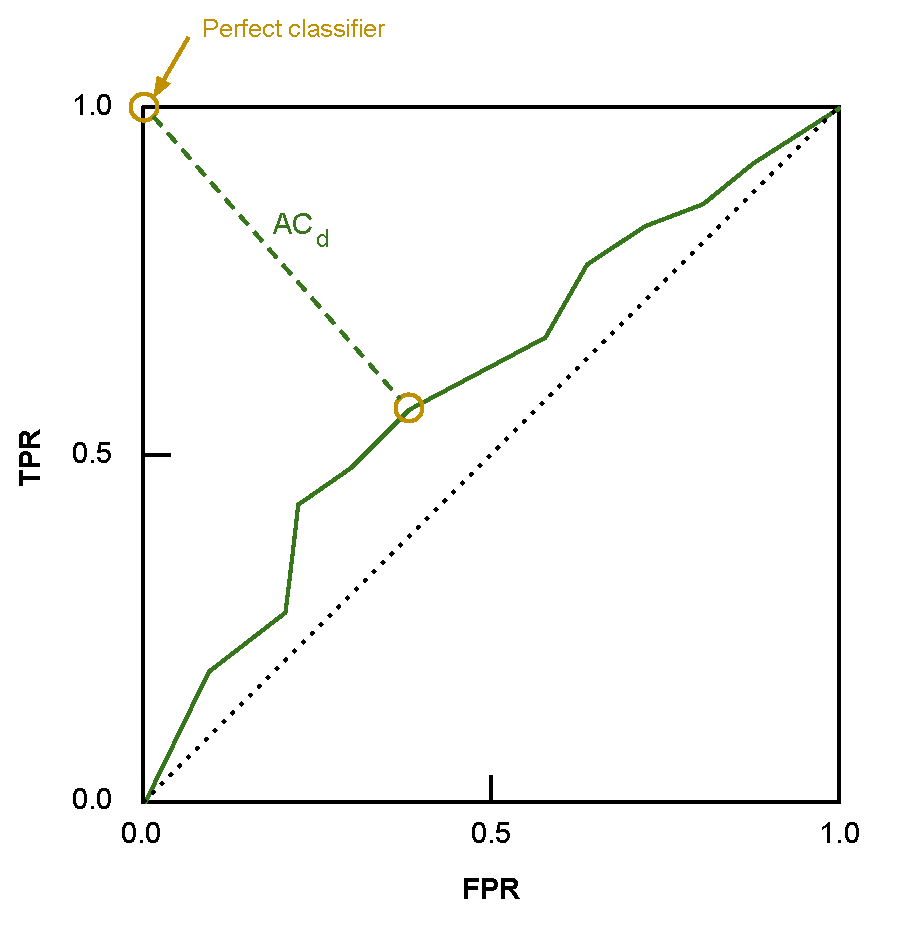
\includegraphics[scale=0.7]{images/roc.pdf}
\caption{ROC (receiving operator characteristics) curve. The $AC_d$ is the distance from a classifier's performance to that of a perfect classifier.}
\label{fig:roc}
\end{figure}

We still lack a single measure that could be used for ranking different classifiers. Since a perfect classifier is the point (0,1) on the ROC curve, we can rank the classifiers based on their distance to that point. Euclidean distance is defined as
\begin{equation}
\text{AC}_d = \sqrt{W \cdot (1 - \text{TPR})^2 + (1 - W) \cdot \text{FPR}^2}, \label{eq:acd}
\end{equation}
where the parameter $W \in [0,1]$ assigns relative importance to false positives and false negatives. The value of $\text{AC}_d$ ranges from 0 for a perfect classifier to $\sqrt{2}$ for a completely incorrect one. \cite{Hamilton12}

To summarize, the parameter selection process goes like this:
\begin{enumerate}
\item{Get parameters values one by one from the grid of available values}
\item{Calculate performance using cross validation and $\text{AC}_d$ as performance measure}
\item{Choose the parameters values with the best performance (highest accuracy or lowest $\text{AC}_d$)}
\end{enumerate}

\subsection{Computational Performance}
Computational performance is not one of the key concerns of this thesis but it is still worth reviewing the possible bottlenecks and ways to improve performance. Not only can the amount of data be huge in CEP, but also the latency with which it is moving should be minimal. That said, our system is of no use if it cannot keep up with new sensor data coming in.

At the core of our system is the Esper CEP Engine which, according to its documentation \cite{EsperReference}, can manage over 500,000 events per second on a dual-core CPU 2 GHz processor with engine latency being less than 3 microseconds on average. The processor on our own test machine is a quad-core CPU 2.5 GHz processor so the performance should be at least at the same level.

It is important to note that training the model does not need to be real-time. In a real-life application the model is trained with regular intervals as a background process. While a new model is being trained, the old model can continue predicting. When the new model is ready, the old model is replaced with it. For example, in our test house this could be done once a month when the indoor air conditions have changed because of, for instance, seasonal changes in the weather.

The prediction phase, in turn, has to be fast as new measurements are coming in all the time. With our DTW and kNN model the prediction includes calculating the DTW distance with each of the training vectors and then selecting \emph{k} closest ones. With our Wavelet and SVM model the prediction phase consists of the Haar Wavelet transform that produces a feature vector and support vector evaluation that classifies the feature vector.

Our computation performance tests evaluate the models' time complexity with respect to window sizes and the number of testing samples. Also the average execution times for classifying a single instance are measured.




